% !TEX TS-program = xelatex
% !TEX encoding = UTF-8 Unicode 

% \documentclass[AutoFakeBold]{LZUThesis}
\documentclass[AutoFakeBold]{LZUThesis}
\usepackage{multirow}
\usepackage{threeparttable}
\CTEXsetup[name={第,部分}]{chapter}
\lstset{
language = MATLAB,
backgroundcolor=\color{white},   % choose the background color; you must add \usepackage{color} or \usepackage{xcolor}  
basicstyle=\footnotesize,        % the size of the fonts that are used for the code  
breakatwhitespace=false,         % sets if automatic breaks should only happen at whitespace  
breaklines=true,                 % sets automatic line breaking  
captionpos=bl,                    % sets the caption-position to bottom  
% commentstyle=\color{green},    % comment style  
% deletekeywords={...},            % if you want to delete keywords from the given language  
% escapeinside={\%*}{*)},          % if you want to add LaTeX within your code  
extendedchars=true,              % lets you use non-ASCII characters; for 8-bits encodings only, does not work with UTF-8  
frame=shadowbox,                    % adds a frame around the code  
keepspaces=true,                 % keeps spaces in text, useful for keeping indentation of code (possibly needs columns=flexible)  
keywordstyle=\color{blue},       % keyword style  
% language=Python,                 % the language of the code  
morekeywords={*,...},            % if you want to add more keywords to the set  
numbers=left,                    % where to put the line-numbers; possible values are (none, left, right)  
numbersep=5pt,                   % how far the line-numbers are from the code  
numberstyle=\tiny\color{gray}, % the style that is used for the line-numbers  
rulecolor=\color{black},         % if not set, the frame-color may be changed on line-breaks within not-black text (e.g. comments (green here))  
showspaces=false,                % show spaces everywhere adding particular underscores; it overrides 'showstringspaces'  
showstringspaces=false,          % underline spaces within strings only  
showtabs=false,                  % show tabs within strings adding particular underscores  
stepnumber=1,                    % the step between two line-numbers. If it's 1, each line will be numbered  
stringstyle=\color{orange},     % string literal style  
tabsize=2,                       % sets default tabsize to 2 spaces  
% title=signalAnalysis.m           % show the filename of files included with \lstinputlisting; also try caption instead of title  
}  

\begin{document}
%=====%
%
%封皮页填写内容
%
%=====%

% 标题样式 使用 \title{{}}; 使用时必须保证至少两个外侧括号
%  如: 短标题 \title{{第一行}},  
% 	      长标题 \title{{第一行}{第二行}}
%             超长标题\tiitle{{第一行}{...}{第N行}}

\title{{对手机价格分层的模型预测}}



% 标题样式 使用 \entitle{{}}; 使用时必须保证至少两个外侧括号
%  如: 短标题 \entitle{{First row}},  
% 	      长标题 \entitle{{First row}{ Second row}}
%             超长标题\entitle{{First row}{...}{ Next N row}}
% 注意:  英文标题多行时 需要在开头加个空格 防止摘要标题处英语单词粘连.

\author{\CJKfontspec{楷体}李文涛}
\major{电子信息基地班}
\college{320200928101}
\grade{2020级}



\maketitle
\frontmatter

%中文摘要
\ZhAbstract{
    本文首先以AMI码为对比对象介绍$\mathrm{HDB_3}$的由来,简略介绍该编码方案的优缺点,
    接着利用MATLAB进行编程,完成对原数字信号序列进行$\mathrm{HDB_3}$编码
    以及后续对信号的频谱分析,对编码
    时频域分析进行谱图可视化,并同时分析其在其传输速率和频谱利用率上的特点。
    最后根据其频谱特性分析其应用价值。
}
{优缺点,MATLAB,时频域分析,应用分析}


%英文摘要
\EnAbstract{This paper introduces the advantages and advantages of $\mathrm{HDB_3}$, 
and then uses MATLAB to program,
 complete the $\mathrm{HDB_3}$ encoding of the original digital signal sequence and the subsequent spectrum analysis of the signal, 
 and the spectral diagram visualization of the encoding time frequency domain analysis, 
 and analyze its characteristics in its transmission rate and frequency utilization.
 Finally, its application value is analyzed according to its spectral characteristics.
    \fontspec{Times New Roman}}
{Advantages and disadvantages, time frequency domain analysis, application analysis}

%生成目录
% \tableofcontents
% \addcontentsline{toc}{chapter}{目录}
% \thispagestyle{empty}


%文章主体
\mainmatter

\chapter{理解数据}

\section{导入数据}

\begin{lstlisting}
    import pandas as pd
    data_test = pd.read_csv('test.csv')
    data_train = pd.read_csv('train.csv')
\end{lstlisting}
将项目处理所需的库和数据集导入。

\section{浏览数据集}

\begin{lstlisting}
    data_test.head()
\end{lstlisting}
用.head()取前五个数据,以用来对数据所包含的信息进行理解。
\begin{figure}[htbp]
    \centering
    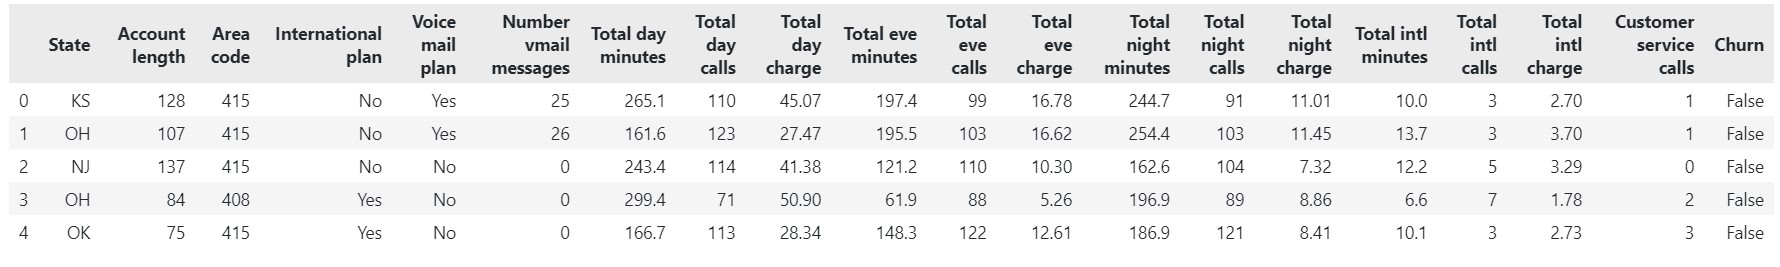
\includegraphics[keepaspectratio,width=500pt]{trainhead.jpg}
    \caption{训练集数据实例}
\end{figure}
\section{对数据属性的理解}
通过上一步我们发现该数据集有$\mathrm{battery\_power}$、$\mathrm{blue}$、$\mathrm{four\_g}$等
一系列属性,通过查阅相关资料,各属性所包含的意思在下方说明。(由于每条数据的属性过多,这里列出部分重要属性)

$\mathrm{battery\_power}$:手机的电池容量

$\mathrm{blue}$:手机是否具有蓝牙功能

$\mathrm{four\_g}$:手机是否具有4G功能

$\mathrm{ram}$:手机的内存容量

$\mathrm{three\_g}$:手机是否具有3G功能

$\mathrm{touch\_screen}$:手机是否为触摸屏

$\mathrm{wifi}$:手机是否具有wifi功能

目标任务为判断测试集手机的$\mathrm{price\_range}$属性。
\chapter{数据清洗}
\section{查看训练集详细信息}
\begin{lstlisting}
    print(data_train.describe())  
\end{lstlisting}
    \begin{figure}[htbp]
        \centering
        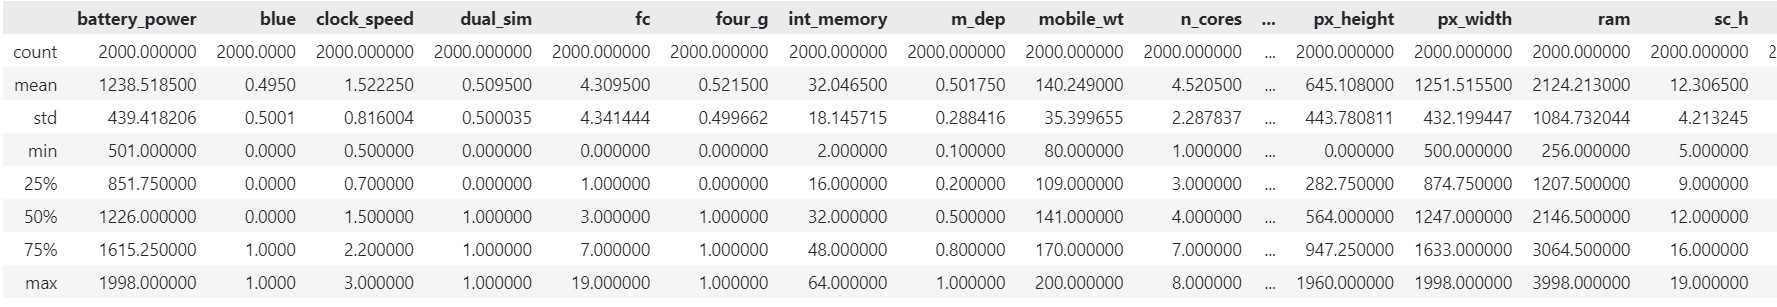
\includegraphics[keepaspectratio,width=450pt]{traindetail.jpg}
        \caption{训练集各数据属性分析}
    \end{figure}
\section{查看数据缺失情况}
\begin{lstlisting}
    print(data_train.info())  
\end{lstlisting}
    \begin{figure}[htbp]
        \centering
        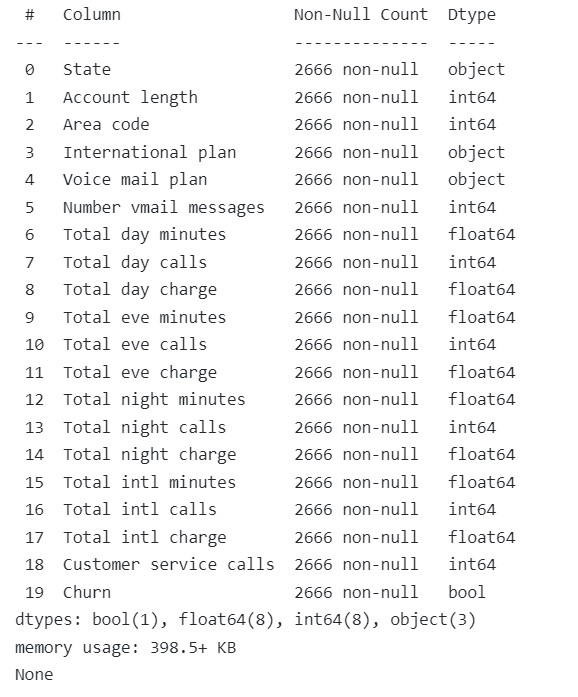
\includegraphics[keepaspectratio,width=160pt]{trainerror.jpg}
        \caption{训练集各数据属性分析}
    \end{figure}

    经观察下图我们发现,各属性数据均完整,且数据类型均为float和int类型,无需多余处理。

\chapter{数据分析}
下面对处理后的数据通过相关直方图和相关系数热力图进行观察比较,选取我们所需要的对手机价格分层的判断属性。

由于数据属性过多,这里我们以$\mathrm{battery\_power}$、$\mathrm{ram}$两属性联合对价格层级$\mathrm{price\_range}$
的影响。

\begin{lstlisting}
    import seaborn as sns 
    import matplotlib.pyplot as plt 
\end{lstlisting}

导入对相关性分析必要的包。

\begin{lstlisting}
    sns.lmplot( data = data_train , x = 'battery_power' ,y = 'ram' , hue = 'price_range');
\end{lstlisting}
\begin{figure}[htbp]
    \centering
    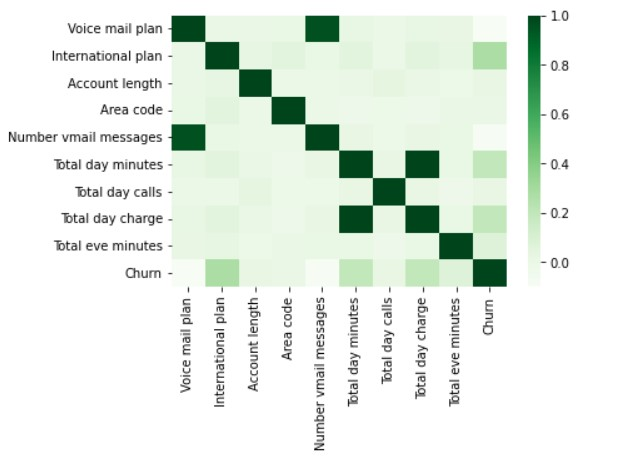
\includegraphics[keepaspectratio,width=320pt]{tconnect.jpg}
    \caption{$\mathrm{battery\_power}$、$\mathrm{ram}$、$\mathrm{price\_range}$的相关关系程度}
\end{figure}
\begin{lstlisting}
    sns.pairplot(data_train)
\end{lstlisting}

利用sns.pairplot函数进一步对所有属性的相关性进行分析,由于导出的图过大,这里将其单独作为
附件导出。

\chapter{构建模型}
考虑到该数据集数据的特殊性,这里采用KNN来进行模型的构建。以下步骤按照参考资料中的代码进行模型的构建。

\section{处理并划分数据集}
\begin{lstlisting}
    # 划分数据集
    data_train_y = data_train.pop('price_range')
    data_train_x = data_train
    from sklearn.model_selection import train_test_split
    X_train,X_test,y_train,y_test = train_test_split(data_train_x,data_train_y,random_state=42)
\end{lstlisting}
这里利用$\mathrm{random\_state}$对每次拆分出的训练集和测试集进行规定,以避免每次数据集的划分随机。
\section{模型训练}
\begin{lstlisting}
    from sklearn.neighbors import KNeighborsClassifier
    model = KNeighborsClassifier(n_neighbors=5)
    model.fit(X_train,y_train)
\end{lstlisting}
\chapter{评估模型}
下面我们分别从混淆矩阵和.score函数来对我们所训练出的模型进行评估。
这里我们将评估这一步骤封装为一个输入模型得出评估的函数,以便之后的进一步改进。
\begin{lstlisting}
    from sklearn.metrics import confusion_matrix,accuracy_score
    def framework(model):
        y_pred = model.predict(X_test)
        cm = confusion_matrix(y_test,y_pred)
        acc = accuracy_score(y_test,y_pred)
        print("ACC:",acc)
        sns.heatmap(cm,annot=True,cmap='Blues')
        plt.show()
\end{lstlisting}
\begin{lstlisting}
    framework(model)
\end{lstlisting}
评估模型。
\begin{figure}[htbp]
    \centering
    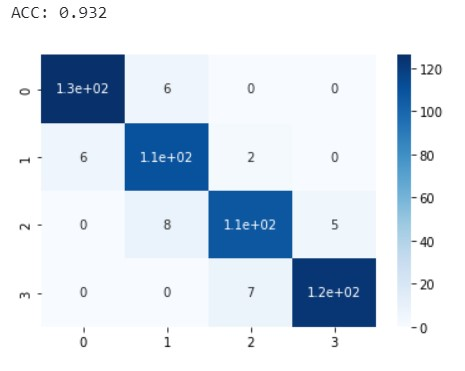
\includegraphics[keepaspectratio,width=280pt]{testframe1.jpg}
    \caption{KNN模型评估结果}
\end{figure}

\chapter{方案改进}
经查阅资料,了解到交叉验证可以提高模型的准确度,以下对KNN模型进行交叉验证的改良。
\begin{lstlisting}
    from sklearn.model_selection import GridSearchCV
    n_neighbors = [5,6,7,8,9,10,11,12,13,14,15,16]
    parameters = dict(n_neighbors=n_neighbors)    
\end{lstlisting}

规定划分参数。
\begin{lstlisting}
    model_improve = GridSearchCV(KNeighborsClassifier(),parameters,cv=10)
    model_improve.fit(X_train,y_train) 
    model_improve.best_score_
    model_improve.best_params_
\end{lstlisting}

调用交叉验证函数,得到交叉验证最佳划分参数和在最佳划分参数下的评估结果。
\begin{lstlisting}
    best_model = model_improve.best_estimator_
    framework(best_model)
\end{lstlisting}
\begin{figure}[htbp]
    \centering
    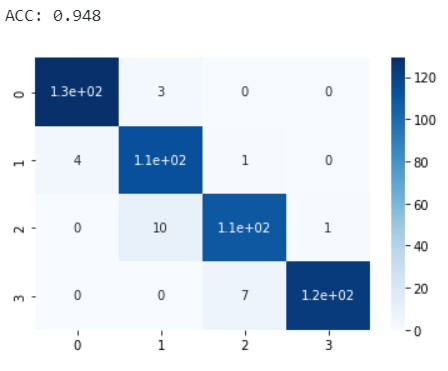
\includegraphics[keepaspectratio,width=280pt]{besttest.jpg}
    \caption{交叉验证后得到的最佳KNN模型评估结果}
\end{figure}
\chapter{方案实施及结果提交}
\begin{lstlisting}
    # 提交数据
    test =  data_test.drop('id',axis=1)
    target = best_model.predict(test)
    price_range = pd.DataFrame(target,columns=['price_range'])
    result = pd.concat([data_test,price_range],axis=1)
    #拼接得到的price_range与测试集
    result.to_csv('result.csv')#输出结果到文件
\end{lstlisting}
\begin{figure}[htbp]
    \centering
    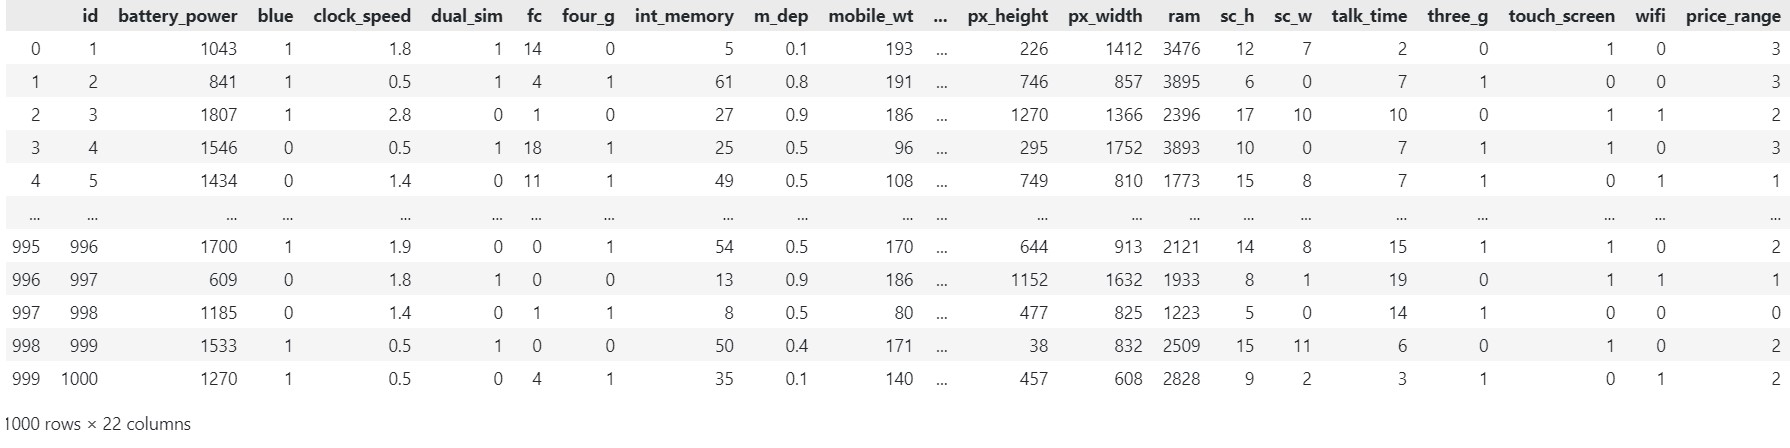
\includegraphics[keepaspectratio,width=450pt]{result.jpg}
    \caption{部分结果输出实例}
\end{figure}
\chapter{总结与收获}
进一步了解了人工智能模型构建的步骤,学习了对模型进一步优化的方法。认识到封装模型构建
函数的不足之处,了解到对于数据的性质,采取不同的模型预测是十分必要的。
\backmatter


% %=======%
% %引入参考文献文件
% %=======%
\bibdatabase{bib/POC}%bib文件名称 仅修改bib/ 后部分
\printbib
\nocite{*} %显示数据库中有的,但是正文没有引用的文献


% \Appendix

% 这里是附录页,可要可不要

% \Thanks.



\end{document}